\documentclass {article}
\usepackage{graphicx}
\usepackage{amsmath}
\usepackage{amssymb}
\usepackage{xcolor}


\renewcommand\vec{\mathbf}
\let\OldS\nabla
\renewcommand{\nabla}{\boldsymbol{\OldS}}

\let\OldHat\hat
\renewcommand{\hat}[1]{\OldHat{\mathbf{#1}}}

% \newcommand{\comment}[1]{}

\newcommand{\comment}[1]{\textcolor{gray}{\small\textit{Comment: #1}}}


\begin{document}
	\thispagestyle{empty}% empty header/footer

	
\begin{center}\strut
	\bfseries\Huge
	What if  Mass Eats the Vacuum? 

\end{center}


\centerline{David Plotz }

\begin{center}\strut
	\date{\today}
	{\today}
\end{center}
\vfill

	
\newpage
\begin{abstract}
	This paper introduces a classical field theory of gravity built on the Maxwell equations and a central hypothesis: that mass absorbs radiation, inducing a net inward momentum flow. We assume a Lorentz-invariant stochastic zero-point radiation field present throughout space and hypothesize that mass acts as a sink for this field.  We construct a consistent model of a massive particle, demonstrate energy and momentum conservation, and show that the three classic tests of general relativity: Mercury's precession, gravitational lensing, and gravitational redshift are reproduced to leading order. This approach provides a novel, Lorentz-invariant, classical alternative to general relativity, and lays a foundation for further exploration.
\end{abstract}
\newpage

\section{Introduction}

 Modern physics rests on two towering achievements: the Standard Model, underpinned by the Dirac equation, and General Relativity, based on Einstein’s field equations. One governs the small, the other the large. Each is remarkably successful in its domain.

But they don’t fit together. When applied simultaneously, the equations break down and yield infinities.  Proposals like string theory offer elegant mathematics but few concrete predictions. Despite nearly a century of effort, no unifying framework has emerged. A fresh approach is warranted.

This paper proposes that fresh approach. Rather than quantizing Einstein’s field equations or geometrizing the Dirac equation, we suggest something simpler and stranger: what if mass eats the vacuum?


\subsection{Roadmap}

This paper is structured to follow the logic of the scientific method: we begin with a hypothesis, outline the assumptions that support it, explore its mathematical consequences, compare its predictions to experiment, and finally examine whether it offers a deeper conceptual shift.

In \textbf{Section 2}, we introduce the hypothesis: that mass acts as a sink for radiation and, in particular, as a sink for a pervasive stochastic zero-point radiation field (Z.P.R.). We first present the idea intuitively, anchoring the theory in a physical picture, and then spell it out mathematically.

In \textbf{Sections 3 and 4}, we lay out the two assumptions underlying the theory. By “assumptions,” we mean elements already present in the scientific literature, perhaps unconventional but not novel to this work. \textbf{Section 3} introduces the stochastic zero-point radiation (Z.P.R.) field as the physical manifestation of the vacuum. \textbf{Section 4} adopts the Maxwell equations as the correct mathematical framework for describing gravity. 

\textbf{Sections 5 and 6} contain the technical core of the paper. We introduce a toy model of a massive particle and discuss characteriscts of the toy model. We examine whether the inflow of radiation can stabilize mass against gravitational self-energy and show that the energy needed for stability of our toy model is less than that available in the Z.P.R.  We also demonstrate conservation of energy and momentum and several other key mathematical results.


In \textbf{Section 7}, we test the theory against observation. We demonstrate that it reproduces the three classic predictions of general relativity to leading order: perihelion precession, gravitational lensing, and redshift.

\textbf{Section 8} explores a surprising result of  the theoory. And finally, \textbf{Section 9} concludes with a discussion of open questions, potential avenues for further investigation, and the broader implications of the framework proposed here.

\section{The Hypothesis}

In this section, we introduce the hypothesis of this paper. Before proceeding, I want to clarify the distinction between assumptions and hypothesis as used here:


\textbf{Assumptions} are drawn from existing theoretical frameworks (even if unconventional). In this paper we make no attempt to prove its claims 
\comment{Claude ... that's not really true ...  In particular, we will be using Heaviside's assumption that we should using the Maxwell equtions ... and we will definitely be examing repurcussions of this assumption, in particular, in relation to the calculations involved in the precession of the perihelion of mercury ... however, with that said, I do want to say, like I'm not trying to defend the Z.P.R. assumptions here ...}

\textbf{Hypothesis} refers to the novel claim proposed in this work

\noindent Every theory begins with a hypothesis. If it yields interesting physics and remains consistent with experiment, it deserves serious consideration. 

Here we first present the hypothesis intuitively, anchoring the theory in a physical picture, and then spell it out mathematically.


\subsection{A Physical Picture: Radiation Sink Intuition }
\label{subsec:intuition}

Before introducing equations, we present a simple physical picture to guide intuition. Consider a neutral, perfectly conducting iron sphere, heated until it glows red. When placed in the vacuum of space, it emits infrared radiation and cools down, eventually approaching absolute zero.

But at zero Kelvin, both classical and quantum theories suggest the presence of a background electromagnetic field called the stochastic zero-point radiation (Z.P.R.) field. A fuller treatment of the Z.P.R. will be offered in \textbf{Section 3}, but for now, it is enough to imagine a low-level radiation noise present even in the coldest vacuum. The iron sphere, after it has cooled down and come into equilibrium with the vacuum, then absorbs radiation from this ambient field.

The hypothesis proposed here is that mass absorbs energy from the zero-point field even at absolute zero. This interaction produces a net inward flow of momentum toward the mass.

The remainder of the paper builds from this intuition and develops the consequences of this idea.



\subsection{Hypothesis: The Math}

The image above anchors the theory.

If mass always interacts with the zero-point field, then this interaction must have physical consequences. We propose it manifests as an inward-pointing momentum density:

\comment{Claude, Is density the right word here?, see eqn \eqref{eq:momentum}}

\begin{equation}
\boxed{\vec{P}(r) = -\hat{r} \frac{G m \hbar}{r^2}}
\label{eq:hypothesis}
\end{equation}


A photon traveling through this field experiences a cumulative momentum shift:

\begin{equation}
\Delta \vec{p} = \int_{\text{path}} \vec{P}(r) \, dl
\label{eq:hypothesis2}
\end{equation}

This is the hypothesis of the paper: mass creates a momentum flux capable of acting on radiation. The implications of this hypothesis will be tested in \textbf{Section 7}.


\section{Zero Point Radiation (ZPR)}

We now introduce our first assumption:  the \textbf{stochastic zero-point radiation field}.  ``Stochastic" means random, in a way that will be clearly defined below, ``zero-point" refers to zero-temperature and ``radiation" in this context simply means light.  


Historically, the Michelson–Morley experiment aimed to detect the luminiferous aether, the medium through which light was thought to propagate. The null result helped solidify the notion of a truly empty vacuum. In contrast, the stochastic zero-point radiation field treats the vacuum as filled with fluctuating electromagnetic fields, even at absolute zero.

This theory was first developed by T.H. Boyer last century but has more interest as of late under the term stochastic electrodynamics (S.E.D.). Stochastic zero-point radiation has been shown to reproduce:
\begin{itemize}
	\item The Planck blackbody spectrum (Boyer, 1969) \cite{boyer1969}
	\item Harmonic oscillator ground-state energy \( \tfrac{1}{2} \hbar \omega \) \cite{cole2003}
	\item Casimir and van der Waals forces \cite{boyer1975}
	\item Certain features of the hydrogen atom’s ground state \cite{puthoff1987}
	\item The Unruh effect \cite{boyer1980}
\end{itemize}

Taken together, these results support the view, held by Boyer and others, that the vacuum is in fact an active medium, filled with fluctuating modes that persist even at \( T = 0 \).  


We therefore, assume that the vacuum is filled with a classical, Lorentz-invariant random electromagnetic radiation field even at absolute zero. The vacuum is not actually empty. It carries a random, omnipresent electromagnetic field with spectral energy density:

\begin{equation}
\rho(\omega) = \frac{1}{2} \hbar \omega
\end{equation}

The zero-point radiation field plays a central role in the framework. The core hypothesis of the theory is that mass interacts with this Z.P.R. field by absorbing momentum from it. 



\subsection{Mathematical Definitions of the Z.P.R.}


The Z.P.R. field is stochastic and Gaussian. The electric and magnetic fields are defined as:

\begin{equation}
\begin{aligned}
\vec{E}(\vec{x}, t) &= \sum_{\lambda=1}^2 \int d^3k \, 
\hat{\epsilon}(\vec{k}, \lambda) 
\sqrt{\frac{\hbar \omega}{8\pi^2}} 
W_\lambda(\vec{k}) e^{i(\vec{k} \cdot \vec{x} - \omega t)} + \text{c.c.}\\
\vec{B}(\vec{x}, t) &= \sum_{\lambda=1}^2 \int d^3k \, 
\frac{\vec{k} \times \hat{\epsilon}(\vec{k}, \lambda)}{|\vec{k}|}
\sqrt{\frac{\hbar \omega}{8\pi^2}} 
W_\lambda(\vec{k}) e^{i(\vec{k} \cdot \vec{x} - \omega t)} + \text{c.c.}
\end{aligned}
\end{equation}

\noindent where $\hat{\epsilon}(\vec{k}, \lambda)$ are polarization vectors satisfying: 

\begin{equation}
\hat{\epsilon} \cdot \vec{k} = 0, \quad
\hat{\epsilon}_1\cdot\hat{\epsilon}_2 = 0, \quad
|\hat{\epsilon}_\lambda| = 1
\end{equation}

\noindent and $W_\lambda(\vec{k})$ are complex Gaussian random variables with correlation properties:

\begin{equation}
\begin{aligned}
\langle W_\lambda(\vec{k}) \rangle &= 0\\
\langle W_\lambda(\vec{k}) W_{\lambda'}^*(\vec{k}') \rangle &= \delta_{\lambda\lambda'} \delta^3(\vec{k} - \vec{k}')\\
\langle W_\lambda(\vec{k}) W_{\lambda'}(\vec{k}') \rangle &= 0
\end{aligned}
\label{eq:stochastic}
\end{equation}

\noindent where $\langle \cdot \rangle$ denotes the stochastic average over the ensemble of random field realizations. This background field is homogeneous, isotropic, and statistically stationary, with the full ensemble remaining invariant under Lorentz transformations.

\subsection{Derivation of Energy Spectrum}

We now verify that this field definition gives the correct energy spectrum. We need to evaluate $\langle \vec{E}^2 \rangle$ and $\langle \vec{B}^2 \rangle$. Let us focus on $\langle \vec{E}^2 \rangle$ as the calculation for the magnetic field is identical.

Write $\vec{E} = \vec{E}_+ + \vec{E}_+^*$ where $\vec{E}_+$ is the positive-frequency part (containing $W_\lambda$ but not $W_\lambda^*$). Then:

\begin{equation}
\vec{E}^2 = (\vec{E}_+ + \vec{E}_+^*)^2 = \vec{E}_+^2 + 2\vec{E}_+ \cdot \vec{E}_+^* + (\vec{E}_+^*)^2
\end{equation}

\noindent Taking the stochastic average:

\begin{equation}
\langle \vec{E}^2 \rangle = 2\langle \vec{E}_+ \cdot \vec{E}_+^* \rangle
\end{equation}

The $\vec{E}_+^2$ and $(\vec{E}_+^*)^2$ terms vanish because $\langle WW \rangle = 0$, by equation \eqref{eq:stochastic}. Evaluating the remaining term:

\begin{equation}
\langle \vec{E}_+ \cdot \vec{E}_+^* \rangle = 
\sum_{\lambda, \lambda'} \int d^3k \, d^3k' \,
\hat{\epsilon}_\lambda \cdot \hat{\epsilon}_{\lambda'}^*
\frac{\hbar\sqrt{\omega\omega'}}{8\pi^2}
\langle W_\lambda(\vec{k}) W_{\lambda'}^*(\vec{k}') \rangle
e^{i(\vec{k} \cdot \vec{x} - \omega t)} e^{-i(\vec{k}' \cdot \vec{x} - \omega' t)}
\end{equation}

\noindent Using the correlation function $\langle W_\lambda(\vec{k}) W_{\lambda'}^*(\vec{k}') \rangle = \delta_{\lambda\lambda'} \delta^3(\vec{k} - \vec{k}')$:

\begin{equation}
\langle \vec{E}_+ \cdot \vec{E}_+^* \rangle = 
\sum_{\lambda} \int d^3k \,
|\hat{\epsilon}_\lambda|^2
\frac{\hbar\omega}{8\pi^2}
\end{equation}

\noindent Since $\sum_{\lambda=1}^2 |\hat{\epsilon}_\lambda|^2 = 2$ (two orthogonal unit polarization vectors):

\begin{equation}
\langle \vec{E}_+ \cdot \vec{E}_+^* \rangle = \int d^3k \, \frac{\hbar\omega}{4 \pi^2}
\end{equation}

\noindent Therefore:

\begin{equation}
\langle \vec{E}^2 \rangle = 2 \int d^3k \, \frac{\hbar\omega}{4 \pi^2}
\end{equation}

\noindent By identical calculation:

\begin{equation}
\langle \vec{B}^2 \rangle = 2 \int d^3k \, \frac{\hbar\omega}{4 \pi^2}
\end{equation}

\noindent The total energy density is:

\begin{equation}
\langle u \rangle = \frac{1}{8\pi}(\langle \vec{E}^2 \rangle + \langle \vec{B}^2 \rangle)
= \frac{1}{8\pi} \cdot 4 \int d^3k \, \frac{\hbar\omega}{4 \pi^2}
= \frac{1}{(2\pi)^3} \int d^3k \, \hbar\omega
\end{equation}

Since $d^3k/(2\pi)^3$ represents the density of states in momentum space (the number of modes per unit volume in $k$-space), we can interpret this as:

\begin{equation}
\langle u \rangle = \int \frac{d^3k}{(2\pi)^3} \, \hbar\omega
= \int [\text{modes per } k^3] \times [\text{energy per mode}]
\end{equation}

This confirms that each electromagnetic normal mode (specified by wavevector $\vec{k}$ and polarization $\lambda$) carries energy $(1/2)\hbar\omega$ in the zero-point radiation field:

\begin{equation}
\boxed{\rho(\omega) = \frac{1}{2} \hbar \omega \quad \text{[energy per mode]}}
\end{equation}

\comment{I have a note here, that like basically maybe I can delete the above two equations ... but will decide on the next editing job.}
\comment {Claude ... I have no idea why it says "[energy per mode]" ... I think maybe deleting the above two simplifies?}
\comment{I haven't actually verified any of these equations in the last chunk of time ... so we really need to do them by pen soon}


\section{Maxwell Equations for Gravity}

In this section we introduce the second of our two assumptions. We call this an assumption because Heaviside first proposed this a long time ago \comment{Claude, Clearly need some reference here and help writing that sentence better}. Following Heaviside, we assume that gravity obeys the same set of  equations as those that govern electromagntism. , up to a numeric factor in the coupling constant. While the Maxwell equations were originally written for charge and charge currents, we replace these with mass and  mass currents acting as sources.  In natural units (\( c = 1 \)):


\begin{equation}
\begin{aligned}
\nabla \times \vec{B} - \partial_t \vec{E} &= -4 \pi G \vec{J}, \quad 
&\nabla \times \vec{E} + \partial_t \vec{B} &= 0 \\
\nabla \cdot \vec{E} &= -4 \pi G \rho, \quad 
&\nabla \cdot \vec{B} &= 0
\end{aligned}
\end{equation}


These equations describe a vector field sourced by mass density \( \rho \) and mass current \( \vec{J} \), with \( G \) the gravitational coupling constant, 6.67 something (Next edit fix this). 

Although derivable from the above, the continuity equation is a useful equation to include here when talking about the Maxwell equations:

\begin{equation}
\nabla \cdot \vec{J}+ \partial_t \rho = 0
\end{equation}

Some may be surprised by the presence of \( \vec{B} \), a magnetic-like field. But this emerges naturally: just as a moving charge generates a magnetic field, a moving mass generates a “gravitomagnetic” field. While static masses generate only \( \vec{E}\), moving masses induce \( \vec{B} \); however, the effect is negligible unless the mass is both extremely large and rapidly moving. \textbf{Section 7} discusses a physical manifestation of this effect and explores its potential testability.

Much of what follows is well-known but are necessary mathematical  tools and techniques that we will use in subsequent sections. 

\subsection{Irrotational and Solenoidal Decomposition}

Any vector field can be split into irrotational (curl-free) and solenoidal (divergence-free) components:

\begin{equation}
\vec{V} = \vec{V}_I + \vec{V}_S, \quad 
\nabla \cdot \vec{V}_S = 0, \quad 
\nabla \times \vec{V}_I = 0
\end{equation}

Applying this to our gravitational fields yields two decoupled subsystems:

\vspace{0.5em}
\noindent\textbf{Static Fields (Irrotational):}

\begin{equation}
\nabla \cdot \vec{E}_I = -4 \pi G \rho, \quad 
\partial_t \vec{E}_I = 4 \pi G \vec{J}_I, \quad 
\nabla \cdot \vec{J}_I + \partial_t \rho = 0
\end{equation}

\noindent\textbf{Radiation Fields (Solenoidal):}


\begin{equation}
\nabla \times \vec{B}_S - \partial_t \vec{E}_S = 4 \pi G \vec{J}_S, \quad 
\nabla \times \vec{E}_S + \partial_t \vec{B}_S = 0
\end{equation}

This decomposition reflects a meaningful physical distinction between the \textbf{static gravitational attraction} and the \textbf{propagating radiation} field. The continuity equation in the irrotational subsystem plays a direct role in what follows.

In the rest frame of the mass, these sectors decouple. One set of equations governs the gravitational field sourced by the mass, while another describes the radiation field. This separation enables a detailed analysis of radiation without affecting the static component. ("Affecting" is the wrong word here?)

We can make this explicit by defining a new current:


\begin{equation}
\vec {J_S'} = - G \vec {J_S}
\end{equation}

\noindent This transforms the inhomogeneous solenoidal equation into:

\begin{equation}
\nabla \times \vec B_S - \partial_t \vec E_S =  4 \pi \vec {J_S'}
\end{equation}

\noindent while leaving all other equations unchanged.

Since this form matches the standard presentation in textbooks on electromagnetic radiation, we will drop the prime and adopt the following as the solenoidal (radiation) Maxwell equations:

\begin{equation}
\begin{aligned}
\nabla \times \vec B_S - \partial_t \vec E_S =  4 \pi \vec J_S \\
\nabla \times \vec E_S + \partial_t \vec B_S = 0 
\end{aligned}
\end{equation}

\subsection{Spherical Vector Harmonics}

Due to the symmetric radial symmetry of the problem, we will benefit from using Vector Spherical Harmonics. 

Following Berrara (http://iopscience.iop.org/article/10.1088/0143-0807/6/4/014/meta) (we should send this to the references when we get a chance) we assume that any vector field, $\vec V$, and any scalar, $g$, can be expanded as follows:



\begin{align}
\vec{V}(\vec{x}) = \sum_{l=0}^{\infty} \sum_{m=-l}^{l} \big[ 
& a_{lm}(r)\, \vec{Y}_{lm}(\theta, \phi) 
+ b_{lm}(r)\, \hat{r} \times \vec{X}_{lm}(\theta, \phi) \notag \\
& + c_{lm}(r)\, \vec{X}_{lm}(\theta, \phi) 
\big]
\end{align}

\begin{equation}
g(\vec x) = \sum_{l=0}^{\infty} \sum_{m=-l}^{l} g_{lm}(r) Y_{lm}(\theta, \phi)
\end{equation}


where $Y_{lm}$ are the usual spherical harmonics (see Jackson 3.53), $\vec Y_{lm}$ is simply $\hat r Y_{lm}$  and $\vec X_{lm}$ is defined as,


\begin{equation}
\vec X_{lm}(\theta, \phi) = \frac {-i}{\sqrt{l(l+1)}} \vec r \times \left( \nabla Y_{lm}(\theta, \phi) \right) 
\label{eq:xlm}
\end{equation}

\subsection{Irrotational Solutions}

We now calculate Newtonian gravity as a solution to the Irrotational parts of the Maxwell equations.

In the case of a static point mass \( m \) located at the origin, (We will have much more to discuss about this in  possibly eqn 52 or 34 ... but they've probably changed R = Gm equation and sigma = m / h delta ) ( we have question marks over here??? ) \comment{we'll fix this up on the next edit} we set:

\begin{equation}
\rho(\vec{x}) = m \delta^3(\vec{x}), \quad \vec{J} = 0
\end{equation}


\noindent Using the irrotational part of the Maxwell equations:


\begin{equation}
\nabla \cdot \vec{E}_I = -4 \pi G \rho ~~~~~~~~~~ \nabla \times \vec{E}_I = 0
\end{equation}

\noindent and using the spherical vector harmonics we developed earlier,  we find:


\begin{equation}
\vec E_I(\vec x) = \sum_{l,m} \left[ -\frac {4\pi i G }{2l+1} \frac {q_{lm}}{r^{l+2}} \sqrt {l(l+1)} \left(\hat r \times \vec X_{lm} \right)  - \frac {4 \pi G (l+1)}{2l+1} \frac {q_{lm}}{r^{l+2}} \vec Y_{lm} \right] 
\end{equation}

\noindent Where,

\begin{equation}
q_{lm} \equiv \int Y_{lm}^* (\theta, \phi) r^l  \rho (\vec x) ~ d^3x = \int \rho_{lm} (r) r^{l+2} ~ dr 
\end{equation}

\noindent Clearly then, if

\begin{equation}
\rho(\vec{x}) = m \delta^3(\vec{x})
\end{equation}


\noindent We get

\begin{equation}
\vec E_I(\vec x) = - \hat{r}\frac {mG} {r^2}
\end{equation}

\noindent as expected.


\subsection{Solenoidal Solutions}
In the last subsection, we derived Newtonian gravity from the irrotational equations, in this subsection we will derive the equations of radiation from teh solenoidal solutions.
Several results from the solutions of the solenoidal Maxwell equations will be needed later; we now solve the corresponding equations.

Outside the mass, the solenoidal field equations in vacuum are:

\begin{equation}
\nabla \times \vec{E}_S + \partial_t \vec{B}_S = 0, \quad 
\nabla \times \vec{B}_S - \partial_t \vec{E}_S = 0
\end{equation}


We write the complete multipole expansion including both electric and magnetic type modes:

\begin{equation}
\begin{aligned}
\vec{B} &= \int d\omega \sum_{l,m} \bigg[
a_E(l,m) f_l(kr) \vec{X}_{lm}
- \frac{i}{k} a_M(l,m) \nabla \times \left( g_l(kr) \vec{X}_{lm} \right)
\bigg] e^{-i\omega t} W_{l,m}(\omega) + \text{c.c.} \\
\vec{E} &= \int d\omega \sum_{l,m} \bigg[
\frac{i}{k} a_E(l,m) \nabla \times \left( f_l(kr) \vec{X}_{lm} \right)
+ a_M(l,m) g_l(kr) \vec{X}_{lm}
\bigg] e^{-i\omega t} W_{l,m}(\omega) + \text{c.c.}
\end{aligned}
\end{equation}

where the functions $f_l$ and $g_l$ are linear superpositions of radial Hankel functions $h_l^{(1)}(kr)$ and $h_l^{(2)}(kr)$, and $W_{l,m}(\omega)$ are complex Gaussian stochastic variables with:

\begin{equation}
\langle W_{l,m}(\omega) \rangle = 0, \quad
\langle W_{l,m}(\omega) W_{l',m'}^*(\omega') \rangle = \delta_{ll'} \delta_{mm'} \delta(\omega - \omega')
\end{equation}

For a massive particle that absorbs radiation (only incoming waves), we have:
\begin{equation}
f_l(kr) = h_l^{(1)}(kr), \quad g_l(kr) = h_l^{(1)}(kr)
\end{equation}

\subsubsection{Computing the Field Momentum}

The total field momentum is:
\begin{equation}
\vec{P}_{\text{field}} = \frac{1}{4\pi } \int_V \vec{E} \times \vec{B} \, d^3x
\end{equation}

\comment{might be an 8 in that denominator}

Following the math we laid out in Section ?, we compute the stochastic average $\langle \vec{E} \times \vec{B} \rangle$. Writing $\vec{E} = \vec{E}_+ + \vec{E}_+^*$ and $\vec{B} = \vec{B}_+ + \vec{B}_+^*$, the terms that survive the stochastic average are those involving $\langle W W^* \rangle$:

\begin{equation}
\langle \vec{E} \times \vec{B} \rangle = \langle \vec{E}_+ \times \vec{B}_+^* \rangle + \langle \vec{E}_+^* \times \vec{B}_+ \rangle
\end{equation}

Working through the cross products using the orthogonality relations of vector spherical harmonics, and noting that $h_l^{(1)*} = h_l^{(2)}$, the angular integrals over $|\vec{X}_{lm}|^2$ yield normalization constants that can be absorbed. 

\begin{equation}
\langle \vec{P}_{\text{field}} \rangle = -\hat{r} \int dr \int d\omega \sum_{l,m} \left[
\frac{-i}{k} |a_E|^2 h_l^{(2)} \frac{1}{r}\frac{d}{dr}\left(r h_l^{(1)}\right)
+ \frac{i}{k} |a_M|^2 h_l^{(1)} \frac{1}{r}\frac{d}{dr}\left(r h_l^{(2)}\right)
\right]
\end{equation}

The above can be simplified by use of the Wronskian, leaving:


\begin{equation}
\boxed{
	\langle \vec{P}_{\text{field}} \rangle = -\hat{r} \int dr \int d\omega \sum_{l,m} \frac{|a_E|^2 |\vec{X}_{lm}|^2}{4\pi k^2 r^2}
}
\label{eq:momentum}
\end{equation}


\subsubsection{Field Energy in the Radiation Zone}

The total field energy density is given by:
\begin{equation}
u = \frac{1}{8\pi}(\vec{E}^2 + \vec{B}^2)
\end{equation}

Computing the stochastically averaged energy density for the full field is complicated due to cross terms between electric and magnetic multipoles. However, in the radiation zone where $k^2 r^2 >> 1$, the fields simplify considerably.

In the radiation zone, using $f_l(kr) \approx h_l^{(1)}(kr) \approx \frac{(-i)^{l+1}}{kr} e^{ikr}$ for incoming waves, the stochastic fields become:

\begin{equation}
\begin{aligned}
\vec{B} &= \frac{e^{ikr}}{kr} \int d\omega \sum_{l,m} (-i)^{l+1} \left[
a_E(l,m) \vec{X}_{lm}
+ a_M(l,m) \hat{r} \times \vec{X}_{lm} 
\right] e^{-i\omega t} W_{l,m}(\omega) + \text{c.c.} \\
\vec{E} &= \frac{e^{ikr}}{kr} \int d\omega \sum_{l,m} (-i)^{l+1} \left[
a_M(l,m) \vec{X}_{lm}
- a_E(l,m) \hat{r} \times \vec{X}_{lm} 
\right] e^{-i\omega t} W_{l,m}(\omega) + \text{c.c.}
\end{aligned}
\end{equation}

Writing $\vec{E} = \vec{E}_+ + \vec{E}_+^*$ and $\vec{B} = \vec{B}_+ + \vec{B}_+^*$, we compute:

\begin{equation}
\langle \vec{E}^2 \rangle = 2\langle \vec{E}_+ \cdot \vec{E}_+^* \rangle, \quad
\langle \vec{B}^2 \rangle = 2\langle \vec{B}_+ \cdot \vec{B}_+^* \rangle
\end{equation}

For $\vec{E}_+ \cdot \vec{E}_+^*$:
\begin{equation}
\langle \vec{E}_+ \cdot \vec{E}_+^* \rangle = \frac{1}{k^2 r^2} \int d\omega \sum_{l,m} 
\left[ |a_M|^2 |\vec{X}_{lm}|^2 + |a_E|^2 |\hat{r} \times \vec{X}_{lm}|^2 \right]
\end{equation}

where the cross terms vanish due to the orthogonality $\vec{X}_{lm} \cdot (\hat{r} \times \vec{X}_{lm}) = 0$.

Similarly:
\begin{equation}
\langle \vec{B}_+ \cdot \vec{B}_+^* \rangle = \frac{1}{k^2 r^2} \int d\omega \sum_{l,m} 
\left[ |a_E|^2 |\vec{X}_{lm}|^2 + |a_M|^2 |\hat{r} \times \vec{X}_{lm}|^2 \right]
\end{equation}

Since $|\hat{r} \times \vec{X}_{lm}| = |\vec{X}_{lm}|$ (both are unit vectors perpendicular to $\hat{r}$), and using the neutrality condition $|a_E|^2 = |a_M|^2$ (see Section~\ref{subsec:intuition}), we obtain:

\begin{equation}
\langle \vec{E}^2 + \vec{B}^2 \rangle = \frac{4}{k^2 r^2} \int d\omega \sum_{l,m} |a_E|^2 |\vec{X}_{lm}|^2
\end{equation}

The total field energy is therefore:

\begin{equation}
\boxed{
	\langle U \rangle = \int_V d^3x \int d\omega \sum_{l,m} \frac{|a_E|^2 |\vec{X}_{lm}|^2}{4\pi k^2 r^2}
}
\label{eq:energy}
\end{equation}

The expansion of this calculation outside the radiation zone involves more intricate mathematics. We defer this more general treatment to future work.




\section{A Toy Model}

In sections three and four, we discussed the assumptions. Up to this point, everything was ground that has been covered by previous researchers. From here on, we rely on new physics. In this section we introduce a module of a massive particle. To gain traction on the problem, we must make  several simplifying assumptions. We hope in future work to study less idealized models.

First, in talking about the space domain, we will quote from Rohrlich at length to find a lower bound for the radius. After, we will move to the frequency domain, and we will speak about the frequency of radiation absorbed by the massive particle (via our hypothesis) and show that for a simple model that only absorbs one frequncy spectra, that we are guaranteed that the massive particle absorbs less energy than is available from the stochastic zero-point radiation field.

\subsection{Lower Bound: Minimum Radius via Gravitational Self-Energy}

The following long quote is from Rohrlich because I can't say it any better than he did. It has been modified from the original to reflect that we are talking about massive particles and not charged particles.

We wish to construct a model of a massive particle. ``The most obvious model of a massive particle is a sphere carrying a spherically symmetrical mass distribution. While such a model is meant (and was indeed proposed) as a picture of a massive elementary particle (a neutron, for example), it is obvious that is is basically a macroscopic massive body, only much smaller. There is nothing 'elementary' about it. To see this clearly, let us consided a macroscopic massive sphere in more detail.

``Consider a sphere of radius $R$ and spherically symmetric mass density $\rho (\vec x)$. Its total mass is
\begin{equation}
m = \int_V \rho(\vec x) d^3x
\end{equation}

``The integral extending over the volume of the sphere. Since $m \neq 0$ by assumption, there must exist attractive gravitational forces between 'parts' of the total mass. Symmetry would therefore require that this massive sphere contract and continue to do so to arbitrarily small radius $R$." Thus with no other forces present, the particle will necessaruly collapse.

Here, it may be prudent to speak about the delta function that we will be uisng. So, if we want to be super technical, the mass distribution would look like:

\begin{equation}
\rho(\vec x) = \frac m {4 \pi r^2} \delta (r - R)
\end{equation}

\noindent But to keep things tidy, we will generally be considering equations where we are "on" the mass shell, so will simply write

\begin{equation}
\rho(\vec x) =  m ~ \delta_{\text{shell}} (\vec x)
\end{equation}



In the next section, I will show that the particle need not collapse. For now, however, let us take it as an assumption that the particle does not collapse. Since we are assuming that there are no other forces in play besides for the gravitational one, its total energy must be

\begin{equation}
U = m = - \frac 1 2 \int \frac {Gm \rho(\vec x)} {r} d^3x
\end{equation}

We note that the more fundamental relativistic expression is $U^2 = m^2$ (or equivalently, $p_\mu p^\mu = m^2$ in four-vector notation), which we utilize and take

\begin{equation}
U^2 = m^2
\end{equation}

To complete the computation, we must choose some mass density distribution to integrate over. Mathematically, following Rohrlich, the simplest is a uniform spherical shell at the radius $R$, in which case

\begin{equation}
m = \frac {Gm^2} { 2R} ~~~~~ or  ~~~~ R = \frac {Gm} 2 
\end{equation}

\comment{Probably flipping the above two equations and be more careful and talk a little about the negative sign}

If, however, we choose a different mass density distribution (a uniform sphere for example), we find that the radius $R$ will always be of the order $Gm$. Therefore, I have chosen $R = Gm$ as the mathematical limit of the radius of a massive particle. This radius is similar in spirit to the classical radius of an electron.

\subsubsection{Macroscopic Objects Aside}

\comment{claude, we need a better title for this subsection }

It is illuminating to compare the mathematical radius with the radii of real physical bodies. Slipping back to SI units, we give a short list of real macroscopice objects with $\Phi = \frac {Gm}{Rc^2}$

$$\text{Mathematical limit:  } ~~~ \Phi = 1 = \frac {Gm}{Rc^2}$$
$$\text{Black hole:  } ~~~ \Phi = 1$$
$$\text{Sun:  } ~~~ \Phi = 2 \times 10^{-6}$$
$$\text{Earth:  } ~~~ \Phi = 7 \times 10^{-10}$$
$$\text{Proton:  } ~~~ \Phi = 1\times 10^{-38}$$


\subsection{Frequency Stuff for our model}
\comment{claude, we need a better title for this subsection }

\comment{Claude, We could mention that boyer has quite a lot to say about a dipole oscillator picking up energy from the Z.P.R. and because Boyer is amazing, he doesn't use this simplified model, but it ends up that he finds that it only picks up frequency from a vary narrow range, so narrow that he might have well as picked the dirac delta that we will introduce. He did the math exactly. But below at least gets to the point ...}

It should be clear that any real model of a macroscopic massive object that absorbs radiation will absorb radiation over a non-singular domain. However, to gain traction, we will suffice with a toy model. We will pick a model that only absorbs one particular frequency. Unsurprisingly, we choose the frequency of light that is absorbed by our massive particle to be



\begin{equation}
	k_{\circ} = \omega_{\circ} = \frac m {\hbar}
\end{equation}

Or, re-writing this as a delta function, in spherical coordinates gives:

\begin{equation}
\frac {\delta \left(\omega - \frac m {\hbar} \right)}{4 \pi \omega^2}
\end{equation}


We can then compute the energy that is absorbed from the field 

\comment {(I'm assuming we have an equation that lines up with this in the stochastic section)}

\begin{equation}
U = \int d\omega  ~~ \hbar \omega  ~ \delta \left(\omega - \frac m {\hbar} \right)
\end{equation}

Which yields 

\begin{equation}
U =  m
\end{equation}

To show that it draws less energy than is available, we will add a constant multiplicative factor \(\alpha\) and re-write the above analysis

\begin{equation}
U =  m = \frac {Gm^2} R
\end{equation}

\noindent and

\begin{equation}
U = \alpha \int \hbar \omega  \delta \left(\omega - \frac m {\hbar} \right)  ~~~ d\omega  
\end{equation}

This yields


\begin{equation}
\alpha = \frac {Gm} R
\end{equation}


\noindent therefore if  \(R > Gm\), which to be clear is what we already showed in the previous section, then \(\alpha < 1\) and we draw less energy from the Z.P.R. than is available.

\subsection{Putting everything together for our model}
Before moving on, we should mention this ``on-shell". So when we deal with the actual equations, we will often be interested in 

\begin{equation}
R = G m
\end{equation}

\noindent and 

\begin{equation}
k_o = \frac m {\hbar}
\end{equation}

\noindent together with the hypothesis at \(r = R\)

\begin{equation}
p = \frac{Gm \hbar} {R^2}
\end{equation}

We can put these all together:

\begin{equation}
\frac{Gm \hbar} {R^2} = \hbar k_o  = m
\end{equation}

\noindent multiplying by \(R/\hbar\) yields

\begin{equation}
\frac{Gm } {R} = k_{\circ} R   = \frac {m R} {\hbar}
\end{equation}

\noindent which yields 

\begin{equation}
k_{\circ} R   = 1
\end{equation}

\noindent and probably more to the point

\begin{equation}
k^2_{\circ} R^2   = 1
\label{eq:kr}
\end{equation}

... In some ways, we shoudn't be too surprised by this result, as we are exactly interested in neither the far limit nor the near limit ... however, it's still pretty cool. And we will call these type of results as being ``on the shell". Finally, as was stated earlier in this section we will use 

\begin{equation}
\delta^{(3)}_{\text{shell}} (\vec x)
\label{eq:dirac_shell}
\end{equation}

\noindent as a simple placeholder to mean ... I mean, really, it means that we will never go in closer than \(R\).


\section{Field Energy and Momentum Balance: A Mechanism for Stability}
\label{sec:stability}

Now that we have laid out \comment{Claude, what's a better way to say "laid out", I think there's something like exposited  ... } our model of a masive particle in the previous section, namely with a shell

\begin{equation}
G m = R
\end{equation}

\begin{equation}
\hbar k_{\circ} = m
\end{equation}

\noindent and

\begin{equation}
k_{\circ} R = 1,
\end{equation}



\noindent we are ready to examine whether the proposed inflow of zero-point radiation can stabilize a massive particle against gravitational collapse. 

Following the ideas of Rohrlich (see the previous section) if the energy absorbed from the vacuum field can offset the divergence in the self-energy of the particle’s own field then we can say that the massive particle is stable against gravitational collapse. We first analyze the energy density and total energy of the system. We then explore whether this energy balance leads to anequilibrium. Finally, we turn to momentum conservation, where we derive an effective “Ohm’s law” relating solenoidal fields and currents. 


\subsection{Stability from Field Energy}

We now evaluate whether the inward radiation flow proposed in \textbf{Section 2} can provide a stabilizing mechanism for a massive particle. Specifically, we ask: can the absorbed energy from the zero-point field counterbalance the gravitational self-energy that would otherwise cause collapse?

The total field energy is given by:
\begin{equation}
U = \frac{1}{16\pi} \int \left( |\vec{E}|^2 + |\vec{B}|^2 \right) \, d^3x
\end{equation}

If we pause and look at just the irrotational part of hese equations, we have

\comment{Well clearly that above sentence was written by a human ... lol}

\begin{equation}
U_I = \frac{1}{16\pi} \int \left( |\vec{E_I}|^2  \right) \, d^3x
\end{equation}

\noindent This leads to 

\begin{equation}
U_I\sim \int \left(\frac { Gm^2} {r^4} \right) \, d^3x
\end{equation}

Which is clearly divergent and therefore a mass would collapse under its own weight without some kind of counter balance force thing.

\comment{Yeah ... I totally used my memory for the above equation, so we should double check it in the next pass}

Unsurprisingly, the hypothesis of this paper is that we should include the radiation contribution, and thus we have:

The total energy, combining both irrotational and solenoidal contributions, is:
\begin{equation}
U_{\text{tot}} = \int_V u \, d^3x = \int_V \left( -\frac{1}{4\pi G} |\vec{E}_I|^2 + |\vec{E}_S|^2 + |\vec{B}_S|^2 \right) \, d^3x
\end{equation}

\noindent Here of course we are "on shell".


From equation~\eqref{eq:energy}, we have:

\begin{equation}
	\langle U \rangle = \int_V d^3x \int d\omega \sum_{l,m} \frac{|a_E|^2 |\vec{X}_{lm}|^2}{4\pi k^2 r^2}
\end{equation}

\comment{This isn't a new equation so shouldn't get it's own number}

Naturally using our hypothesis, we simply write this as  

\begin{equation}
U_{\text{rad}} =  \frac{1}{8\pi^3} \int \int \frac{Gm \hbar}{r^2} \, d^3x \, d^3k
\end{equation}

Integrating over \(k\) and combining, and of course just as we had "numerical prefactors" in section about mass r = R, here we do suppress numerical prefactors and absorb them into the definition of the model. gives the following total energy:

\begin{equation}
U_{\text{tot}} = \int \left[ \frac{Gm \hbar}{r^2}k^3  - \frac {Gm^2} {r^4}\right] \, d^3x 
\end{equation}

Using straightforward algebra with the assumption that we are "on shell", so that \(k = m / \hbar\) and with \(r = R\).  And therefore 


\begin{equation}
U_{\text{tot}} = \int \left[ 0\right] \, d^3x 
\end{equation}


\noindent we then see that the energy is at most a constant and therefore is conseved.


\subsection{Momentum Conservation and “Ohm’s Law”}

We now turn to momentum conservation. The total momentum exchange in the system should obey:

\begin{equation}
\int_V \left( \rho \vec{E}_I + \vec{J}_S \times \vec{B}_S \right) \, d^3x = 0
\end{equation}


Assuming the solenoidal current obeys a linear response:

\begin{equation}
\vec{J}_S = \sigma \vec{E}_S
\end{equation}

And assuming that we use our model, such that (see \eqref{eq:dirac_shell})

\begin{equation}
\rho= m \delta^3 ( \vec{x})
\end{equation}

Averaging over the stochastic noise the field momentum becomes:

\begin{equation}
-\hat{r} \int \left( m \delta^3(\vec{x}) \cdot \frac{G m}{r^2} - \sigma \cdot \frac{G m \hbar}{r^2} \right) \, d^3x = 0
\end{equation}

Solving gives:

\begin{equation}
\sigma = \frac{m}{\hbar} \delta^3(\vec{x})
\end{equation}

This expression defines a delta-function conductivity concentrated at the origin, but knowing we actually mean the shell. Thus this is an effective Ohm's law in which the mass acts as a point-like, perfect absorber for incoming radiation as long as we are outside of the radius \(R\).  We can re-write the relevant Maxwell equation in light of this:

\begin{equation}
\nabla \times \vec{B}_S - \partial_t \vec{E}_S = -\frac{m}{\hbar} \vec{E}_S \delta^3(\vec{x})
\label{eq:ohm}
\end{equation}



Together, the field energy and momentum conservation arguments presented in this section demonstrate that the core hypothesis of momentum inflow can stabilize a massive particle. A massive particle that sinks zero-point radiation does not collapse becauseit can pull energy from the vacuum field itself.

	
\section{Classical Tests of Gravity}

This section demonstrates that the present theory reproduces three key experimental predictions of general relativity: the precession of Mercury's perihelion, the deflection of light near a massive object, and gravitational redshift. 

\comment{These are the three classic tests of general relativity ... like pretty sure that Einstein himself propsed these ... or at minimum ... like they're really famous ... we should double check this, and then also mention this up above in the intro and the conclusion} 

\subsection{Precession of the Perihelion of Mercury}

In electrodynamics, a static Coulomb field transforms under Lorentz boosts into a configuration with both electric and magnetic components. Specifically, the fields of a charge moving at velocity \( \vec{v} \) are:

\begin{equation}
\vec{E}' = \gamma \vec{E} - \frac{\gamma^2}{\gamma + 1} \vec{v} (\vec{v} \cdot \vec{E}), \quad
\vec{B}' = - \gamma \vec{v} \times \vec{E}
\end{equation}

where \( \gamma = 1 / \sqrt{1 - v^2} \).

By analogy, we assume the same Lorentz transformation laws apply to gravity. We define the gravitational field:

\begin{equation}
\vec{E}_g = \vec{F} / m = - \frac{G M}{r^3} \vec{r}
\end{equation}

Then, under a Lorentz boost:

\begin{equation}
\vec{E}_g' = \gamma \vec{E}_g - \frac{\gamma^2}{\gamma + 1} \vec{v} (\vec{v} \cdot \vec{E}_g), \quad
\vec{B}_g' = -\gamma \vec{v} \times \vec{E}_g
\end{equation}

In the low-velocity limit \( v \ll 1 \), we find:

\begin{equation}
\vec{B}_g = - \vec{v} \times \vec{r} \cdot \frac{GM}{r^3}
\end{equation}

This introduces a "gravitomagnetic" interaction analogous to magnetism in electrodynamics.

\begin{figure}[t]
	\centering
	\fbox{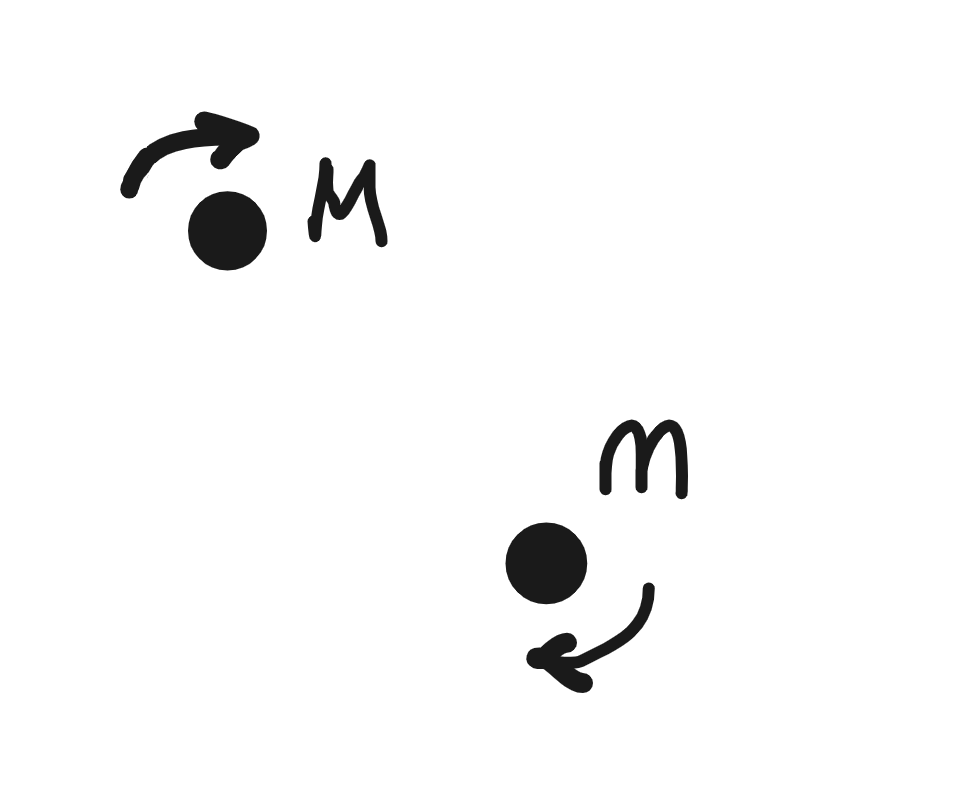
\includegraphics[width=0.6\textwidth]{autodraw.png}}
	\caption{Two masses in mutual orbit}
	\label{fig:two-masses}
\end{figure}

We now consider Kepler’s problem. The Newtonian effective potential is:




\begin{equation}
U_{\text{Newt}} = \frac{1}{2} m \left( \frac{dr}{dt} \right)^2 - \frac{GMm}{r} + \frac{l^2}{2 m r^2}
\end{equation}

where \( l = m |\vec{r} \times \vec{v}| \) is the orbital angular momentum (see Figure \ref{fig:two-masses}).


A moving charge induces a magnetic moment \( \vec{m} = \frac{1}{2} e (\vec{r} \times \vec{v}) \). Replacing \( e \rightarrow m \), we define a gravitational magnetic moment:

\begin{equation}
\vec{m}_g = \frac{1}{2} m (\vec{r} \times \vec{v})
\end{equation}

The potential energy of this moment in a magnetic field is:

\begin{equation}
U = -\vec{m}_g \cdot \vec{B}_g = -\frac{GM m}{2} |\vec{r} \times \vec{v}|^2 / r^3
\end{equation}

This adds a correction to the potential energy. Including the reciprocal effect (from the motion of the central mass), we double this term and find the corrected potential:

\begin{equation}
U_{\text{Einstein}} = \frac{1}{2} m \left( \frac{dr}{dt} \right)^2 - \frac{GMm}{r}
+ \frac{l^2}{2 m r^2} - \frac{GM l^2}{m r^3}
\end{equation}

This is the same correction obtained in general relativity to first order. As Carroll notes, general relativity produces this result exactly; in our theory, it emerges as a first-order approximation. Higher-order terms may offer a route to testing deviations.

\subsection{Deflection of Light}



We now consider the deflection of light near a massive object. Our central hypothesis is that mass creates a momentum-transfer field:

\begin{equation}
\vec{P}(r) = - \hat{r} \frac{G m \hbar}{r^2}
\tag{\ref{eq:hypothesis}}
\end{equation}


\begin{figure}[h]
	\centering
	\fbox{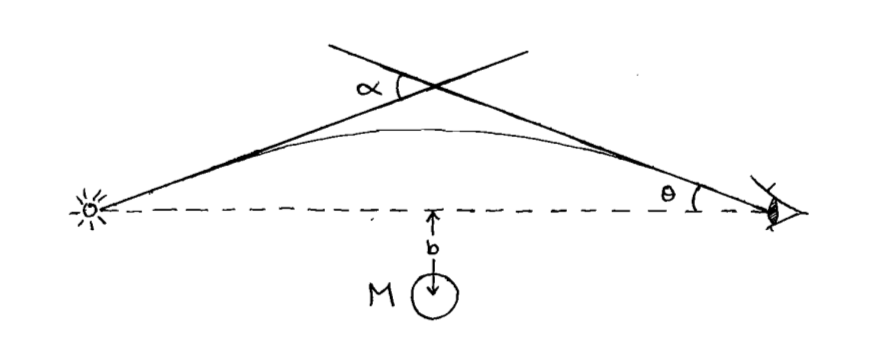
\includegraphics[width=0.6\textwidth]{light-bending.png}}
	\caption{Deflection of light}
	\label{fig:deflection}
\end{figure}

A photon traveling through this field receives a cumulative momentum shift:

\begin{equation}
\Delta \vec{p} = \int_{\text{path}} \vec{P}(r) \, dl
\tag{\ref{eq:hypothesis2}}
\end{equation}

Assuming a straight-line path passing at minimum distance \( b \) (see figure \(\ref{fig:deflection}\)), we integrate:

\begin{equation}
\Delta \vec{p} = \int_{-\infty}^{\infty} - \frac{G m \hbar}{r^3} \vec{r} \, w \, dz
\end{equation}

The parallel momentum shifts cancel symmetrically. The transverse component yields:

\begin{equation}
\Delta p_y = \hbar w \cdot \frac{2 G m}{b}
\end{equation}

The angle of deflection is then:

\begin{equation}
\theta \approx \frac{\Delta p_y}{p_z} = \frac{2 G m}{b} \quad \Rightarrow \quad \alpha = \frac{4 G m}{b}
\end{equation}

This matches, to first-order, the deflection angle predicted by general relativity.

\subsection{Gravitational Redshift}

Finally, we consider the redshift of light climbing out of a gravitational well. As before, a photon gains or loses momentum depending on its path through the momentum field.

Using:

\begin{equation}
\Delta p = \int_{\infty}^{R} \vec{P} \cdot \hat{r} \cdot w \, dr = \int_{\infty}^{R} - \frac{G m \hbar}{r^2} w \, dr = \hbar w \cdot \frac{G m}{R}
\end{equation}

The resulting frequency shift is:

\begin{equation}
\hbar w' = \hbar w + \Delta p = \hbar w \left( 1 + \frac{G m}{R} \right)
\end{equation}

which, to first order, matches the prediction of general relativity for gravitational redshift.

		
\section{Duality and the Dirac Equation}

Throughout this paper, we’ve stayed grounded in classical physics. We built a theory of gravity using field equations, conservation laws, and an underlying sea of vacuum radiation: no quantum assumptions, no curved spacetime. In this section, something surprising appears. When the field equations are rewritten in a new form, a familiar structure emerges: the Dirac equation, the cornerstone of quantum mechanics.

\subsection{Duality Transformations}

As discussed in Jackson (Section 6.11), the Maxwell equations can be extended to include both electric and magnetic charges:

\begin{equation}
\begin{aligned}
\nabla \times \vec{B} - \partial_t \vec{E} &= \vec{J}_e, \quad
&\nabla \times \vec{E} + \partial_t \vec{B} &= -\vec{J}_m \\
\nabla \cdot \vec{E} &= \rho_e, \quad
&\nabla \cdot \vec{B} &= \rho_m
\end{aligned}
\end{equation}


The magnetic densities are assumed to obey the same continuity equation as their electric counterparts.

Now consider the following duality transformation:

\begin{equation}
\begin{aligned}
\vec{E} &= \vec{E}' \cos \xi + \vec{B}' \sin \xi, \quad
&\vec{B} &= \vec{B}' \cos \xi - \vec{E}' \sin \xi \\
\rho_e &= \rho_e' \cos \xi + \rho_m' \sin \xi, \quad
&\rho_m &= \rho_m' \cos \xi - \rho_e' \sin \xi \\
\vec{J}_e &= \vec{J}_e' \cos \xi + \vec{J}_m' \sin \xi, \quad
&\vec{J}_m &= \vec{J}_m' \cos \xi - \vec{J}_e' \sin \xi
\end{aligned}
\end{equation}


This transformation leaves the generalized Maxwell equations invariant. As Jackson notes, the distinction between electric and magnetic charge is, in this framework, a matter of convention. If all particles share the same magnetic-to-electric charge ratio, a duality rotation can eliminate magnetic charges entirely. This perspective opens the door for deeper reinterpretations of classical field theory.

\subsection{Spinor Representation of Field Operators}

We now examine a way to recast Maxwell’s equations using spinor-like objects.

Define the vector curl as a matrix operator:

\begin{equation}
\nabla \times \vec{V} = g_i \partial_i \vec{V}
\end{equation}

with:

\begin{equation}
g_1 = \begin{pmatrix}
0 & 0 & 0 \\
0 & 0 & -1 \\
0 & 1 & 0
\end{pmatrix}, \quad
g_2 = \begin{pmatrix}
0 & 0 & 1 \\
0 & 0 & 0 \\
-1 & 0 & 0
\end{pmatrix}, \quad
g_3 = \begin{pmatrix}
0 & -1 & 0 \\
1 & 0 & 0 \\
0 & 0 & 0
\end{pmatrix}
\end{equation}

Define the gamma matrices as (These matrices satisfy the algebra of infinitesimal rotations and generate the curl operator in 3D”):

\begin{equation}
\gamma^0 = \begin{pmatrix}
-1 & 0 \\
0 & -1
\end{pmatrix}, \quad
\gamma^i = \begin{pmatrix}
0 & g_i \\
-g_i & 0
\end{pmatrix}
\end{equation}

These matrices are not the standard Dirac representation, but they serve to connect the structure of the field equations to the spinor formalism in a suggestive way. This could be further explored with tools from representation theory and Clifford algebras.

\subsection{Emergence of the Dirac Equation}

Recall from the section on momentum conservation that we have quation~\eqref{eq:ohm}:

\begin{equation}
\nabla \times \vec{B}_S - \partial_t \vec{E}_S = -\frac{m}{\hbar} \vec{E}_S \delta^3(\vec{x})
\tag{\ref{eq:ohm}}
\end{equation}

Restricting attention to the surface of the particle (i.e., “on-shell”) as explained several times in several places ... \comment{Sorry for getting kind of snarky here ... The first time I gave this paper to Claude, Claude was quite insistent on making this super explicit}

Therefore we drop the delta function and write:

\begin{equation}
\nabla \times \vec{B}_S - \partial_t \vec{E}_S = -\frac{m}{\hbar} \vec{E}_S
\end{equation}

Now, apply the duality transformation and write the solenoidal Maxwell equations in this form:

\begin{equation}
\begin{aligned}
-\partial_t \vec{E}_S + \nabla \times \vec{B}_S + \frac{m}{\hbar} \vec{E}_S &= 0 \\
-\partial_t \vec{B}_S - \nabla \times \vec{E}_S + \frac{m}{\hbar} \vec{B}_S &= 0
\end{aligned}
\end{equation}

Using the spinor curl definition:

\begin{equation}
\begin{aligned}
-\partial_t \vec{E}_S + g_i \partial_i \vec{B}_S + \frac{m}{\hbar} \vec{E}_S &= 0 \\
-\partial_t \vec{B}_S - g_i \partial_i \vec{E}_S + \frac{m}{\hbar} \vec{B}_S &= 0
\end{aligned}
\end{equation}


Now define a six-component field:

\begin{equation}
\psi = \begin{pmatrix}
\vec{E}_S \\
\vec{B}_S
\end{pmatrix}
\end{equation}

We can combine the two equations above into a compact form:

\begin{equation}
\left( \gamma^\mu \partial_\mu + \frac{m}{\hbar} \right) \psi = 0
\end{equation}

This has the exact form of the Dirac equation, as given in Sakurai’s Advanced Quantum Mechanics, Eq. 3.31.

The matrices $g_i$ defined here are the standard generators of SO(3) rotations—the antisymmetric 3x3 matrices representing infinitesimal rotations in three-dimensional space. The representation $\nabla \times \vec{V} = g_i \partial_i \vec{V}$ can be verified by direct computation: the curl operation naturally emerges from the commutation relations of these generators. While this is not the standard Dirac representation (which operates on four-component spinors in Minkowski space), it serves to express the Maxwell curl operations in a form that makes the structural similarity to the Dirac equation manifest. The resulting six-component field  $ \psi = (\vec{E}_S, \vec{B}_S)^T $ is not a quantum spinor but a classical field object.

This is a remarkable result: starting from classical field equations and a single added hypothesis, we arrive at a spinor field satisfying the Dirac equation. This is of course done without quantization or any reference to spin. 


\section{Conclusion}


\comment{The next three paragraphs, ChatGPT helped me write ... they sound like ChatGPT wrote them ... Hopefully, we can make this sound more human in a new draft}

Can gravity emerge from classical physics, without invoking curved spacetime or quantum gravity? That was the question we asked. Faced with two powerful but incompatible theories, quantum mechanics and general relativity, we chose a different path: to treat mass as a source of momentum flow, drawing from a pervasive background field. The result is a framework that is simple, classical, and deeply physical.

To test the idea, we built the theory step by step. We formulated equations for how mass interacts with the vacuum field. We introduced cutoffs to make the interaction finite and consistent. We checked for conservation of energy and momentum. Then we asked: does this theory match observation? And the answer, to leading order, is yes. It reproduces the familiar predictions of general relativity: the bending of light, gravitational redshift, and the precession of Mercury.

But something unexpected happened. When we re-expressed the field equations in a different form, they gave rise to the Dirac equation, the same equation that governs quantum particles like electrons. This wasn’t assumed; it emerged. That a single classical field framework can describe gravity, electromagnetism, and quantum behavior is remarkable. It suggests these aren’t separate layers of physics, but different faces of the same underlying structure. One set of equations that does it all.

\comment{The below line I like a lot}

 This stands in contrast to general relativity, where mass is treated as a cold object sitting in empty space and curving spacetime around it


\subsection{Where This Could Go}

The assumption that mass sinks radiation is implicit in the Feynman Lectures. ... but we are making it our "core" hypothesis?

Here, in the current iteration of this paper, we simply state the hypothesis and explore its consequences. In future drafts or subsequent work, we hope to derive this form directly from the two assumptions laid out in the next sections.


Several directions remain open:

- \textbf{Expansion of the energy outside of the radiation zone} As mentioned in the text, surrounding equation \ref{eq:energy}, it would be interesting to expand this energy equation to ouside of the radiation zone.

- \textbf{Expansion of the precession of the perihelion Calculation} If we went to higher order in this calculation, we could have a simple test to test the difference ... This was probably explained in the text.

- \textbf{Removal of the Hypothesis} As mentioned in the text \textbf{Section ?}, it is the belief of this author that we can actually derive the hypothesis from the assumptions.  Then this theory wouldn't even need an hypothesis.

- \textbf{RLess Idealized Models}  Currently our model of a massive particle is as simple as possible. It would be interesting to study less idealized models.


\subsection{Final Thought}

Physicists have long sought simplicity. Apparently the universe is built on simple laws. Einstein advised making a theory as simple as possible, but no simpler. When a single framework explains more with less, it earns our attention. Bringing electricity, magnetism, gravity, and the Dirac equation under one set of equations is a level of simplicity that deserves serious attention.

The history of physics is full of bold guesses. Some are wrong, some are premature, and some are foundational. This is just a guess. But it is a specific, testable, and mathematically structured one. If nothing else, it shifts the question. Gravity need not emerge from geometry. It might instead arise from the quiet hiss of radiation no one thought to listen to.

This is offered not as a conclusion, but as a beginning. Collaborators welcome.


\section*{Acknowledgments}

This paper would not exist without the support of a few key people. First and foremost, I thank my wife, who has stood beside me for over two decades as I pursued this idea. Her patience, steadiness, and quiet encouragement through all the ups and downs have been unwavering.

I am also deeply grateful to my friend Michael Seidel, who, despite not having a background in physics, listened to me explain these ideas again and again over the years. His willingness to engage, ask questions, and simply be present helped me find clarity when I needed it most.

To both of them: thank you.



\begin{thebibliography}{99}
	

	
\end{thebibliography}

\end{document}